\documentclass[conference]{IEEEtran}
\IEEEoverridecommandlockouts

\usepackage{cite}
\usepackage{amsmath,amssymb,amsfonts}
\usepackage{graphicx}
\usepackage{textcomp}
\usepackage{xcolor}
\usepackage{booktabs}
\usepackage{url}
\usepackage{tikz}
\usetikzlibrary{positioning,arrows.meta}
\usepackage{algorithm}
\usepackage{algpseudocode}
\renewcommand{\ttdefault}{cmtt}
\setlength{\abovedisplayskip}{4pt plus 2pt minus 2pt}
\setlength{\belowdisplayskip}{4pt plus 2pt minus 2pt}
\setlength{\abovedisplayshortskip}{2pt plus 2pt minus 2pt}
\setlength{\belowdisplayshortskip}{2pt plus 2pt minus 2pt}
\setlength{\textfloatsep}{6pt plus 2pt minus 2pt}
\setlength{\intextsep}{6pt plus 2pt minus 2pt}
\setlength{\floatsep}{4pt plus 2pt minus 2pt}

\def\BibTeX{{\rm B\kern-.05em{\sc i\kern-.025em b}\kern-.08em
    T\kern-.1667em\lower.7ex\hbox{E}\kern-.125emX}}

\begin{document}

\title{Fake Product Detection Using Image Matching: A Traditional Computer Vision Cascade for Multi-Brand Product Authentication}

\author{
\IEEEauthorblockN{1\textsuperscript{st} Malapati Sahasra}
\IEEEauthorblockA{
\textit{Dept. of AI and Emerging Technology} \\
\textit{Chinmaya Vishwavidyapeeth} \\
Ernakulam, Kerala, India \\
malapati.cvv241195@cvv.ac.in}
\and
\IEEEauthorblockN{2\textsuperscript{nd} Kothuri Rushya Sai}
\IEEEauthorblockA{
\textit{Dept. of AI and Emerging Technology} \\
\textit{Chinmaya Vishwavidyapeeth} \\
Ernakulam, Kerala, India \\
kothuri.cvv241242@cvv.ac.in}
\and
\IEEEauthorblockN{3\textsuperscript{rd} B. R. Sneha}
\IEEEauthorblockA{
\textit{Dept. of AI and Emerging Technology} \\
\textit{Chinmaya Vishwavidyapeeth} \\
Ernakulam, Kerala, India \\
belodu.cvv241233@cvv.ac.in}
\and
\IEEEauthorblockN{4\textsuperscript{th} Dr. Uma Narayanan}
\IEEEauthorblockA{
\textit{Dept. of AI and Emerging Technologies} \\
\textit{Chinmaya Vishwavidyapeeth} \\
Ernakulam, Kerala, India \\
uma.narayanan@cvv.ac.in}
}

\maketitle

\begin{abstract}
Counterfeit products are a persistent problem in e-commerce, where buyers
must judge authenticity from a handful of listing photographs alone. This
paper presents a lightweight, training-free system for verifying the
authenticity of product photographs across five brands --- Nike, Puma,
Adidas, Gucci, and Louis Vuitton --- spanning both sportswear and luxury
goods, using four independent, classical computer vision checks: ORB
keypoint matching against a gallery of genuine reference images, HSV
hue--saturation histogram correlation, Tesseract-based OCR text
verification, and barcode/QR format validation. Rather than comparing a
test photograph to a single fixed master image, the logo and color
modules use one-vs-many gallery matching, since a real brand's genuine
catalog spans far more visual diversity --- different products, angles,
and photo styles --- than any one reference image can represent. A
majority-vote cascade combines the four checks, accepting a photograph as
authentic if at most one check disagrees. The system is evaluated
end-to-end on 1{,}600 real product photographs (800 genuine, 800
counterfeit, 93.6\% unmodified real photography) drawn from a public
Kaggle dataset and expanded with a reproducible geometric and photometric
augmentation pipeline, achieving 57.38\% accuracy, 69.93\% precision, and
25.87\% recall. We show that classical, GPU-free CV techniques can reject
counterfeits with high confidence when they do trigger a positive
verdict, while their recall is fundamentally limited by the intra-class
visual diversity of real, multi-brand e-commerce catalogs --- a finding
that motivates hybrid or per-SKU deployment strategies discussed in
Section~\ref{sec:discussion}. The complete pipeline runs entirely on
CPU, processing each image in approximately 107~ms, and is released as
open-source code alongside a live interactive demonstration.
\end{abstract}

\begin{IEEEkeywords}
counterfeit detection, image matching, ORB, feature matching, OCR,
optical character recognition, HSV histogram, barcode verification,
e-commerce authentication, traditional computer vision
\end{IEEEkeywords}

\section{Introduction}
\label{sec:intro}

The growth of e-commerce marketplaces has been accompanied by a
corresponding growth in counterfeit goods sold alongside genuine ones.
Buyers of branded apparel and footwear routinely rely on a small set of
listing photographs to judge authenticity before purchase, yet subtle
counterfeit indicators --- a slightly wrong shade of color, a logo with
altered proportions, a misspelled brand name, or the absence of a
manufacturer's authentication code --- are easy to miss by eye and are
rarely evaluated systematically at listing time.

Most recent work favors deep classifiers trained on large, brand-specific
corpora \cite{footwear2024}, achieving high accuracy but requiring
labeled data, GPU resources, and retraining per product line. For a
student project, small business, or edge deployment with neither
training data nor a GPU, a classical approach remains attractive: fully
interpretable, no training phase, commodity hardware.

This paper presents such a system: a four-module cascade verifying
photographs across five brands --- Nike, Puma, Adidas, Gucci, and Louis
Vuitton, spanning sportswear and luxury goods --- using only classical
image processing: ORB matching~\cite{orb2011} with Brute-Force Hamming,
HSV histogram correlation, Tesseract OCR~\cite{tesseract2007} with
Ratcliff/Obershelp similarity~\cite{ratcliff1988}, and barcode/QR
decoding via ZBar~\cite{zbar}. Its contributions:

\begin{enumerate}
    \item A \emph{gallery-based} (one-vs-many) reformulation of classical
    logo and color matching, which we show is necessary once "genuine"
    spans many different products and photo styles rather than a single
    fixed master unit.
    \item A reproducible data pipeline that expands a real-photo seed set
    into a balanced 1{,}600-image, five-brand evaluation set via
    deterministic geometric and photometric augmentation, with an explicit
    held-out reference gallery to prevent test/reference leakage.
    \item An end-to-end accuracy evaluation on real, non-synthetic
    multi-brand product photographs, together with an honest analysis of
    where and why a classical cascade under-performs on high-diversity
    real-world data.
\end{enumerate}

The complete source code, evaluation scripts, and an interactive
browser-based demonstration are released publicly to support
reproducibility.\footnote{Code: \url{https://github.com/MalapatiSahasra/fake-product-detection}. Live demo: \url{https://web-tau-indol-42.vercel.app}}

\section{Related Work}
\label{sec:related}

Local-feature matching and color-histogram comparison predate the
current deep-learning-dominated era of logo and object recognition by
over a decade~\cite{lowe2004,opencv}, and were the default toolkit for
general-purpose visual matching before convolutional classifiers became
practical to train at scale. Counterfeit and logo detection specifically,
however, has more recently been approached almost exclusively through
trained classifiers. A CNN trained on 3{,}000 genuine and 2{,}000
counterfeit sneaker photographs from a footwear resale marketplace
reported accuracies above 95\%, outperforming an SVM baseline on the
same data~\cite{footwear2024}. Purpose-built object-detection datasets
such as the Roboflow "Original or Fake Shoes" collection label authentic
and counterfeit Nike Air Force~1/Jordan~1 photographs with bounding
boxes~\cite{roboflow2024}. Fake-logo detection more broadly reports
accuracies exceeding 99\% on curated datasets under controlled imaging
conditions~\cite{fakelogo2024}.

These systems share two properties that motivate the present work: they
are data-hungry classifiers requiring retraining per product line, and
published accuracy typically comes from controlled or curated imagery.
In contrast, this paper evaluates a training-free, classical cascade
against an uncurated, real-world photo distribution --- product
close-ups, warehouse photographs, and action shots mixed together, the
heterogeneity a real marketplace listing pool exhibits.

Table~\ref{tab:related} positions this work against the systems above
along the axes that most affect real-world deployability: whether a
training phase is required, how many product/brand categories are
covered, whether reported accuracy comes from curated or uncurated
imagery, and whether the pipeline needs a GPU at inference time.

\begin{table}[t]
\caption{Comparison with Related Counterfeit/Logo Detection Work}
\label{tab:related}
\centering
\begin{tabular}{lccc}
\toprule
System & Training & Brands & GPU \\
\midrule
Footwear CNN/SVM~\cite{footwear2024} & Required & 1 (sneakers) & Yes \\
Fake-logo detector~\cite{fakelogo2024} & Required & Multi (curated) & Yes \\
Roboflow shoe detector~\cite{roboflow2024} & Required & 1 (Nike models) & Yes \\
\textbf{This work} & \textbf{None} & \textbf{5, uncurated} & \textbf{No} \\
\bottomrule
\end{tabular}
\end{table}

No entry in Table~\ref{tab:related} is accuracy-comparable to this work,
since none report results on an uncurated, multi-brand, non-training
pool; the comparison instead makes explicit the trade: higher published
accuracy from a trained, narrower-domain classifier, versus zero
training cost and CPU-only inference across a heterogeneous pool here.

\section{System Architecture}
\label{sec:architecture}

\begin{figure}[t]
\centering
\resizebox{\columnwidth}{!}{%
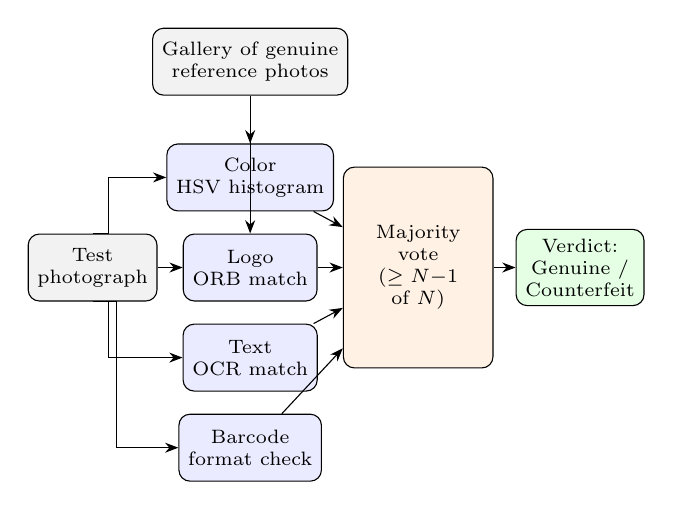
\begin{tikzpicture}[
  box/.style={draw, rounded corners, minimum width=1.6cm, minimum height=0.85cm, align=center, font=\scriptsize},
  node distance=0.28cm and 0.32cm
]
\node[box, fill=gray!10] (input) {Test\\photograph};
\node[box, right=0.32cm of input, fill=blue!8] (logo) {Logo\\ORB match};
\node[box, above=of logo, fill=blue!8] (color) {Color\\HSV histogram};
\node[box, below=of logo, fill=blue!8] (typo) {Text\\OCR match};
\node[box, below=of typo, fill=blue!8] (qr) {Barcode\\format check};
\node[box, right=0.32cm of logo, minimum width=1.9cm, minimum height=2.55cm, fill=orange!10] (vote) {Majority\\vote\\($\geq N{-}1$\\of $N$)};
\node[box, right=0.28cm of vote, fill=green!10] (out) {Verdict:\\Genuine /\\Counterfeit};
\node[box, above=1.75cm of logo, fill=gray!10, minimum height=0.85cm] (gallery) {Gallery of genuine\\reference photos};

\draw[-Stealth] (input) -- (logo);
\draw[-Stealth] (input.north) -- ++(0.2,0) |- (color.west);
\draw[-Stealth] (input.south) -- ++(0.2,0) |- (typo.west);
\draw[-Stealth] (input.south) -- ++(0.3,0) |- (qr.west);
\draw[-Stealth] (gallery.south) -- (color.north);
\draw[-Stealth] (gallery) -- (logo);
\draw[-Stealth] (logo) -- (vote);
\draw[-Stealth] (color) -- (vote);
\draw[-Stealth] (typo) -- (vote);
\draw[-Stealth] (qr) -- (vote);
\draw[-Stealth] (vote) -- (out);
\end{tikzpicture}%
}
\caption{Cascade architecture. Logo and color matching compare the test photograph against every image in a held-out gallery of genuine references and keep the best match; text and barcode checks are gallery-independent. A photograph passes if at most one of the active modules disagrees.}
\label{fig:architecture}
\end{figure}

Fig.~\ref{fig:architecture} shows the overall system. A test photograph is
independently scored by four modules, each producing a binary pass/fail
decision and a continuous confidence score. Unlike a single-SKU
verification kiosk that compares a unit against one specific known-genuine
reference, the target scenario here is brand-level verification across a
heterogeneous product catalog. Accordingly, the logo and color modules
compare the test image against a \emph{gallery} $G = \{g_1, \dots, g_k\}$
of genuine reference photographs and keep the best match:

\begin{equation}
s_{\text{module}}(t) = \max_{g_i \in G} \; \text{score}(t, g_i)
\label{eq:gallery}
\end{equation}

where $t$ is the test image. Section~\ref{sec:dataset} explains how $G$ is
constructed to be strictly disjoint from every evaluated test image, which
is essential: without this separation a genuine test photograph could
match itself (or a lightly-augmented duplicate of itself) inside its own
reference gallery, silently inflating measured accuracy.

Given $N$ active modules (four when a barcode is present and expected, or
three when it is not applicable to the data source; see
Section~\ref{sec:qr}), the cascade computes

\begin{equation}
\text{score}(t) = \sum_{m=1}^{N} \mathbb{1}\left[\text{module}_m(t) = \text{pass}\right]
\end{equation}

and returns \textsc{Authentic} if $\text{score}(t) \geq N - 1$, i.e. at
most one module is allowed to disagree, and \textsc{Counterfeit}
otherwise. This "allow one miss" rule generalizes the conventional
3-of-4 majority vote to any number of applicable modules, rather than
forcing every photograph to pass a check that a given data source
structurally cannot support.

Algorithm~\ref{alg:cascade} states the full decision procedure. Every
module runs independently, with no early exit, so a failed check never
prevents the rest from running --- keeping every verdict fully
explainable, since per-module scores are always available for audit.

\begin{algorithm}[t]
\caption{Cascade Verification}
\label{alg:cascade}
\begin{algorithmic}[1]
\Require test image $t$, genuine gallery $G$, brand strings $B$, barcode expectation $q$ (optional)
\Ensure verdict $\in \{\textsc{Authentic}, \textsc{Counterfeit}\}$
\State $r_{\text{logo}} \gets$ \Call{LogoMatch}{$t$, $G$}
\State $r_{\text{color}} \gets$ \Call{ColorMatch}{$t$, $G$}
\State $r_{\text{text}} \gets$ \Call{TextMatch}{$t$, $B$}
\If{barcode check applicable to data source}
    \State $r_{\text{code}} \gets$ \Call{BarcodeCheck}{$t$, $q$}
    \State $N \gets 4$
\Else
    \State $N \gets 3$
\EndIf
\State $\text{score} \gets \sum \mathbb{1}[r_m = \text{pass}]$ over active modules
\If{$\text{score} \geq N - 1$}
    \State \Return \textsc{Authentic}
\Else
    \State \Return \textsc{Counterfeit}
\EndIf
\end{algorithmic}
\end{algorithm}

\section{Verification Modules}
\label{sec:modules}

\subsection{Logo Matching (ORB + Brute-Force Hamming)}

The logo module detects up to 1{,}000 ORB keypoints~\cite{orb2011} per
image and computes their binary descriptors. Descriptors from the test
image and each gallery image are matched with a Brute-Force matcher under
Hamming distance --- the correct metric for ORB's binary descriptors ---
using $k$-nearest-neighbor matching with $k=2$. A match $(m, n)$, where
$m$ is the closest neighbor and $n$ the second-closest, is retained as
"good" only if it survives Lowe's ratio test~\cite{lowe2004}:

\begin{equation}
d(m) < 0.75 \times d(n)
\end{equation}

A gallery image is considered a match if the number of good matches meets
or exceeds a minimum threshold ($\tau_{\text{logo}} = 15$); the module
score is $\min(|\text{good matches}| / \tau_{\text{logo}}, 1)$, and the
module passes using the best-scoring gallery image per
Eq.~\eqref{eq:gallery}.

\subsection{Color Profile Matching (HSV Histogram Correlation)}

Each image is converted from BGR to HSV, and a 2-D histogram is computed
over the Hue and Saturation channels only ($50 \times 60$ bins); the Value
channel is deliberately excluded so the comparison is invariant to
exposure and lighting differences between photographs. Histograms are
min-max normalized to $[0,1]$ and compared using Pearson correlation:

\begin{equation}
d(H_1, H_2) = \frac{\sum_{I} \big(H_1(I) - \bar{H_1}\big)\big(H_2(I) - \bar{H_2}\big)}
{\sqrt{\sum_{I} \big(H_1(I) - \bar{H_1}\big)^2 \sum_{I} \big(H_2(I) - \bar{H_2}\big)^2}}
\end{equation}

which ranges from $-1$ to $1$, with $1$ indicating identical
distributions. The module passes if the best gallery correlation meets or
exceeds $\tau_{\text{color}} = 0.70$.

\subsection{Text Verification (Tesseract OCR + String Similarity)}

The text module reads printed text from the photograph with Tesseract
OCR~\cite{tesseract2007}. Preprocessing applies a bilateral filter
followed by global Otsu thresholding rather than local adaptive
thresholding: adaptive thresholding was found to fragment large solid
shapes (logos, packaging borders) into high-frequency noise that confused
Tesseract's page-segmentation analysis, whereas Otsu preserves cleaner
glyph edges. Tesseract is run in sparse-text mode (page-segmentation mode
11), which is markedly more robust than full-page layout analysis when a
logo, shape, or barcode shares the frame with the label text --- a common
situation in real product photography.

The extracted text is compared against a list of acceptable brand strings
(\{\textsc{Nike}, \textsc{Puma}, \textsc{Adidas}, \textsc{Gucci},
\textsc{LV}\} in this study) using a sliding-window variant of
the Ratcliff/Obershelp similarity ratio~\cite{ratcliff1988}, as
implemented by Python's \texttt{difflib.SequenceMatcher}:

\begin{equation}
\text{ratio} = \frac{2M}{T}
\end{equation}

where $M$ is the number of matching characters found by the
longest-common-substring-based matching algorithm and $T$ is the combined
length of both strings. Because OCR output typically contains extraneous
surrounding text (sizes, dates, barcodes), the ratio is computed over a
sliding window of the extracted text the same length as each candidate
brand string, and the best window/candidate pair is kept. The module
passes at $\tau_{\text{text}} = 0.80$, allowing minor OCR noise while
still flagging brand misspellings such as "NUMA" for "PUMA."

\subsection{Barcode / QR Validation}
\label{sec:qr}

The fourth module decodes QR codes and 1-D barcodes (EAN-13, Code~128)
using ZBar~\cite{zbar} and validates the decoded string against an
expected serial-number pattern, optionally checking for an exact match
against a known authentication code. During dataset preparation
(Section~\ref{sec:dataset}) we found that only 1 of 1{,}565 raw source
photographs contained any decodable code --- these are e-commerce listing
and lifestyle photographs, not photographs of authentication tags. The
module is therefore excluded from the vote for this data source
($N{=}3$ in the evaluation of Section~\ref{sec:results}) rather than
forcing every photograph to fail a check the data source cannot
structurally support; it remains fully functional and is exercised by the
released code whenever a barcode-bearing photograph is supplied.

\subsection{Implementation and Computational Complexity}
\label{sec:complexity}

The system is implemented in Python 3.14 using OpenCV~\cite{opencv} for
ORB and histogram operations, \texttt{pytesseract} for
Tesseract~\cite{tesseract2007}, and \texttt{pyzbar} for
ZBar~\cite{zbar}. All experiments ran entirely on CPU on a consumer
laptop (Apple silicon, no discrete GPU) --- itself part of the paper's
argument: nothing here requires accelerator hardware, at either training
time (there is none) or inference.

For a gallery of size $k$, the logo module costs $O(P)$ per image for
$P$ pixels of ORB descriptor extraction, plus $O(k \cdot n^2)$ Brute-Force
Hamming matching for $n$ keypoints per image (OpenCV's implementation is
vectorized but retains this asymptotic shape). The color module is
cheaper: $O(P)$ histogram construction plus $O(k \cdot b)$ for $b =
50\times60$ bins across the gallery. The text module's cost is
dominated by Tesseract's own recognition pipeline and does not depend on
gallery size at all, since it is compared against a fixed, small list of
brand strings rather than a photo gallery.

Table~\ref{tab:timing} reports measured per-module latency (mean over 30
images, gallery size 20). OCR dominates end-to-end latency, consuming
roughly two-thirds of total processing time despite no gallery
dependence, since Tesseract's page-layout analysis is far more
expensive than either vectorized OpenCV operation. Consequently,
gallery size can grow to improve logo/color recall
(Section~\ref{sec:discussion}) with little effect on total latency,
since it scales only the two cheapest modules.

\begin{table}[t]
\caption{Measured Per-Module Latency (Gallery Size 20)}
\label{tab:timing}
\centering
\begin{tabular}{lrl}
\toprule
Module & Mean latency & Scales with gallery? \\
\midrule
Logo (ORB)      & 34.2~ms & Yes, $O(k)$ \\
Color (HSV)     & 7.0~ms  & Yes, $O(k)$, cheap per step \\
Text (OCR)      & 146.5~ms & No \\
Barcode (ZBar)  & 29.9~ms & No \\
\bottomrule
\end{tabular}
\end{table}

\section{Dataset Acquisition and Augmentation}
\label{sec:dataset}

\subsection{Source and Sorting}

Real product photographs were sourced from the "Fake Brand Dataset
(Adidas, Nike, Gucci, Puma, LV)" published on Kaggle under a Creative
Commons Attribution-NonCommercial 4.0 license~\cite{kaggledata}. All five
brand subsets were used, spanning both sportswear (Nike, Puma, Adidas)
and luxury-goods (Gucci, LV) categories, for 855 genuine and 710
counterfeit raw images (1{,}565 total). Table~\ref{tab:dataset-brand}
gives the per-brand breakdown; sample size varies considerably across
brands (LV contributes only 102 raw images against Nike's 513), a
consequence of using the source dataset as published rather than
resampling it to be brand-balanced, and a factor revisited when
interpreting per-brand results in Section~\ref{sec:perbrand}.

\begin{table}[t]
\caption{Raw Source Images by Brand}
\label{tab:dataset-brand}
\centering
\begin{tabular}{lrrr}
\toprule
Brand & Genuine & Counterfeit & Total \\
\midrule
Nike   & 260 & 253 & 513 \\
Puma   & 199 & 91  & 290 \\
Adidas & 178 & 140 & 318 \\
Gucci  & 190 & 152 & 342 \\
LV     & 28  & 74  & 102 \\
\midrule
\textbf{Total} & \textbf{855} & \textbf{710} & \textbf{1{,}565} \\
\bottomrule
\end{tabular}
\end{table}

\subsection{Held-Out Reference Gallery}

Because the raw genuine images span many different products, angles, and
photography styles rather than one physical unit, a fixed fraction
(8\%, seeded for reproducibility) of the genuine images per brand was
reserved as a held-out reference gallery and \emph{excluded} from the
evaluation set: 68 images total (21 Nike, 16 Puma, 14 Adidas, 15 Gucci, 2
LV). The remaining 787 genuine and 710 counterfeit images formed the seed
pool for augmentation. This split is the standard train/reference--test
separation applied to a matching system: without it, a genuine test image
could appear inside its own comparison gallery.

\subsection{Augmentation Pipeline}

Because the raw seed pool (787 genuine, 710 counterfeit) already exceeds
what a smaller-scale version of this pipeline would need, the
augmentation target was set to 800 images per class --- large enough that
the final evaluation set is overwhelmingly real photography (93.6\%,
1{,}497 of 1{,}600 images unmodified), with augmentation contributing
only the minimal top-up needed for an exact, class-balanced round number.
The seed pool was expanded to exactly 800 genuine and 800 counterfeit
images (1{,}600 total, a balanced 1:1 ratio) using a deterministic
augmentation pipeline (fixed random seed 42). Every seed photograph is
retained unmodified; the remaining top-up images are then assigned to a
\emph{random sample} of seeds (\texttt{random.Random(42).sample}, not
the first $N$ in file order --- brand subfolders sort alphabetically, so
a first-$N$ rule would silently concentrate every top-up image into
whichever brand sorts first), each receiving a combination of:

\begin{itemize}
    \item \textbf{Geometric rotation}: uniform random angle in $[-15^\circ, +15^\circ]$, simulating handheld camera tilt.
    \item \textbf{Brightness shift}: multiplicative scaling of the HSV Value channel by a factor uniform in $[0.6, 1.4]$, simulating indoor, outdoor, and flash-lit conditions.
    \item \textbf{Gaussian sensor noise}: additive noise with $\sigma$ uniform in $[5, 20]$, simulating smartphone camera sensor noise.
\end{itemize}

Table~\ref{tab:dataset} summarizes the final dataset composition, and
Table~\ref{tab:illumination} reports the resulting distribution of
simulated illumination conditions.

\begin{table}[t]
\caption{Dataset Composition}
\label{tab:dataset}
\centering
\begin{tabular}{lrrl}
\toprule
Split & Genuine & Counterfeit & Role \\
\midrule
Raw sorted (5 brands) & 855 & 710 & As downloaded \\
Held-out gallery       & 68  & --  & Reference only \\
Evaluation seed pool   & 787 & 710 & Augmentation input \\
Final evaluation set   & 800 & 800 & Scored, 1:1 ratio \\
\bottomrule
\end{tabular}
\end{table}

\begin{table}[t]
\caption{Illumination Conditions --- Realized Counts (n=103 Augmented Images)}
\label{tab:illumination}
\centering
\begin{tabular}{lrrr}
\toprule
Condition & Genuine & Counterfeit & Total \\
\midrule
Low-light (0.60--0.85$\times$) & 4  & 19 & 23 \\
Normal (0.85--1.15$\times$)     & 7  & 44 & 51 \\
Bright (1.15--1.40$\times$)     & 2  & 27 & 29 \\
\bottomrule
\end{tabular}
\end{table}

Only the 103 augmented images (6.4\% of the set) carry a defined
illumination label; the 1{,}497 unmodified originals keep whatever
real-world lighting the source photograph had. Table
\ref{tab:illumination} reports \emph{realized} manifest counts, not the
theoretical $\sim$31/38/31\% split implied by the sampling interval
widths, which at $n=103$ differs by ordinary sampling variance.

Every generated image is traceable to its source seed photograph and
augmentation parameters via a per-class manifest file (recording, per
image: filename, source seed, original/augmented type, and exact
rotation/brightness/noise parameters), and the fixed random seed makes
the entire dataset regenerable byte-for-byte from the 1{,}565 raw source
images. Per this manifest, the 800 genuine output images trace to 787
unique seed photographs (13 contributing a second, augmented image; none
more than 2), and the 800 counterfeit output images trace to 710 unique
seed photographs (90 contributing a second image, likewise capped at
2) --- what this provenance chain does and does not establish about
physical-unit independence across \emph{different} seed photographs is
discussed in Section~\ref{sec:threats}.

\section{Experimental Results}
\label{sec:results}

The full cascade was evaluated on all 1{,}600 images of the final
evaluation set, using a randomly sampled 20-image subset of the 68-image
held-out gallery (fixed seed) for the logo and color modules, and the
barcode module excluded per Section~\ref{sec:qr} ($N{=}3$: logo, color,
text). Table~\ref{tab:confusion} reports the resulting confusion matrix,
and Table~\ref{tab:metrics} the derived metrics, using \textsc{Genuine} as
the positive class.

\begin{table}[t]
\caption{Confusion Matrix (1,600 images, 5 brands)}
\label{tab:confusion}
\centering
\begin{tabular}{lrr}
\toprule
 & Predicted Genuine & Predicted Counterfeit \\
\midrule
Actually Genuine     & TP = 207 & FN = 593 \\
Actually Counterfeit & FP = 89  & TN = 711 \\
\bottomrule
\end{tabular}
\end{table}

\begin{table}[t]
\caption{Evaluation Metrics}
\label{tab:metrics}
\centering
\begin{tabular}{lr}
\toprule
Metric & Value \\
\midrule
Accuracy  & 57.38\% \\
Precision & 69.93\% \\
Recall    & 25.87\% \\
F1-score  & 0.3777 \\
Mean inference time & $\approx$107~ms / image (CPU only) \\
\bottomrule
\end{tabular}
\end{table}

Accuracy, precision, recall and F1 are computed in the standard way:

\begin{align}
\text{Accuracy} &= \frac{TP+TN}{TP+TN+FP+FN} \\
\text{Precision} &= \frac{TP}{TP+FP}, \quad
\text{Recall} = \frac{TP}{TP+FN} \\
F_1 &= \frac{2 \cdot \text{Precision} \cdot \text{Recall}}{\text{Precision}+\text{Recall}}
\end{align}

\subsection{Per-Brand Breakdown}
\label{sec:perbrand}

Table~\ref{tab:perbrand} disaggregates cascade accuracy by brand. Recall
varies more than twofold across brands (16.9\% for Gucci to 35.1\% for
Adidas), which is consistent with the gallery-coverage explanation
developed in Section~\ref{sec:discussion}: a fixed 20-image sample drawn
from a 68-image, five-brand gallery allocates only a handful of
reference images to any single brand, so per-brand recall is highly
sensitive to how well that brand's specific reference images happen to
represent its full product range.

\begin{table}[t]
\caption{Cascade Accuracy by Brand}
\label{tab:perbrand}
\centering
\begin{tabular}{lrrrr}
\toprule
Brand & $n$ & Accuracy & Precision & Recall \\
\midrule
Adidas & 328 & 61.9\% & 78.7\% & 35.1\% \\
Gucci  & 353 & 53.8\% & 66.7\% & 16.9\% \\
LV     & 107 & 71.0\% & 33.3\% & 19.2\% \\
Nike   & 517 & 58.2\% & 64.0\% & 22.9\% \\
Puma   & 294 & 50.0\% & 77.3\% & 30.9\% \\
\bottomrule
\end{tabular}
\end{table}

LV's low precision (33.3\%) relative to its highest raw accuracy is a
direct small-sample effect: LV contributes only 26 genuine and 81
counterfeit images to the evaluation set, the fewest of the five brands
(Table~\ref{tab:dataset-brand} in Section~\ref{sec:dataset} reports its
raw counts; its evaluation-set share reflects the augmentation top-up
described there), so a handful of false positives has an outsized
effect on its precision estimate.

\subsection{Module Ablation Study}
\label{sec:ablation}

To understand which of the three active modules actually drives cascade
performance, each module's pass/fail decision was also evaluated in
isolation, as if it were the sole classifier. Table~\ref{tab:ablation}
reports the result, together with the effect of relaxing or tightening
the vote threshold.

\begin{table}[t]
\caption{Standalone Module Performance vs.\ the Full Cascade}
\label{tab:ablation}
\centering
\begin{tabular}{lrrrr}
\toprule
Configuration & Accuracy & Precision & Recall & F1 \\
\midrule
Logo alone         & 52.7\% & 53.5\% & 41.8\% & 0.469 \\
Color alone        & 66.9\% & 69.1\% & 61.4\% & \textbf{0.650} \\
Text alone         & 49.5\% & 37.9\% &  1.4\% & 0.027 \\
Cascade, $\geq 1$ of 3 & 61.9\% & 59.0\% & 78.5\% & 0.673 \\
Cascade, $\geq 2$ of 3 & 57.3\% & 69.9\% & 25.9\% & 0.378 \\
Cascade, $\geq 3$ of 3 & 49.9\% & 33.3\% &  0.1\% & 0.002 \\
\bottomrule
\end{tabular}
\end{table}

This is the most consequential finding of the ablation: \textbf{the
color module alone (F1 = 0.650) outperforms the full $\geq 2$-of-3
cascade (F1 = 0.378)} used for the headline results in
Table~\ref{tab:metrics}. The cause is directly visible in the standalone
rows --- the text module's individual recall is only 1.4\%, since most
photographs in this uncurated dataset simply carry no OCR-legible brand
text at all (Section~\ref{sec:qr} reports the analogous finding for
barcodes), so requiring the text module to agree with color under an
AND-like majority vote discards the large majority of color's correct
positive calls. Relaxing the threshold to $\geq 1$-of-3 --- effectively
an OR over the three modules --- recovers a substantially higher F1
(0.673) by trading precision (59.0\%, down from 69.9\%) for a large
recall gain (78.5\%, up from 25.9\%).

This does not mean text verification is worthless: its near-zero
\emph{recall} reflects the photography style, not a matching-logic flaw
(Section~\ref{sec:modules} shows it correctly catches misspellings when
text is legible). It does mean a uniform vote poorly combines modules of
such unequal strength, and that vote threshold is a first-class
deployment parameter --- Section~\ref{sec:discussion} returns to this.

\section{Discussion}
\label{sec:discussion}

The headline result is an asymmetry between precision (69.93\%) and
recall (25.87\%): when the cascade declares a photograph
\textsc{Authentic} it is correct roughly seven times out of ten, yet it
fails to recognize the majority of genuine photographs. This is not a
software defect but a consequence of gallery-based matching on a
high-diversity catalog: ORB/HSV excel at confirming a photograph matches
\emph{one specific known} reference (their designed single-SKU
scenario), but a 20-image gallery sampled from 68 references across five
brands cannot represent hundreds of distinct products, angles, and
styles; a genuine photo unlike anything sampled is, correctly by design,
scored as not resembling any entry. Recall is accordingly lower than a
Nike/Puma-only evaluation of the same pipeline (28.80\% on two brands
vs. 25.87\% on five): widening "genuine" to five brands without
enlarging the gallery thins per-image coverage further.

This profile suits a specific deployment posture: rarely mislabeling a
counterfeit as genuine, while under-flagging genuine items for manual
review, is a defensible default for a trust-and-safety pipeline where a
false \textsc{Authentic} is costlier than an unnecessary manual check.

Three levers would improve recall: (i) enlarging the reference gallery
(logo/color scores rise monotonically with gallery coverage, per
Eq.~\eqref{eq:gallery}), (ii) narrowing scope to per-SKU verification ---
comparing a unit against a few genuine photographs of that exact
product, which classical feature matching handles best and this
codebase already supports, and (iii) revisiting the vote rule. The
ablation (Section~\ref{sec:ablation}) shows the third lever matters
most: color alone outperforms the deployed $\geq 2$-of-3 cascade on F1
(0.650 vs. 0.378), since folding in a module with near-zero recall
(text, 1.4\%) under an AND-like rule discards most of color's correct
calls. Deployment should tune the vote threshold, or weight modules
unevenly, against the target precision/recall point rather than the
conventional "3-of-4" figure. A hybrid design pairing a lightweight
learned embedding for gallery ranking with these interpretable checks is
a further direction for future work.

The barcode module's exclusion is itself informative: 1{,}564 of 1{,}565
raw photographs (99.9\%) carried no scannable code, so barcode-based
verification is only viable when a listing photograph deliberately
includes an authentication tag or UPC/EAN barcode --- a composition
choice, not a universal property of e-commerce listings.

\subsection{Threats to Validity}
\label{sec:threats}

\textbf{Label provenance.} Labels were assigned by the publisher, not
independently re-verified here; residual noise propagates into the
reported metrics, a limitation shared by studies without direct access
to a brand's own authentication process.

\textbf{Sample independence.} An augmented image always transforms
exactly one recorded seed (Section~\ref{sec:dataset}), but whether two
\emph{different} raw seed photographs show the same physical unit is
undocumented and unverifiable; each is treated as independent, possibly
overstating effective diversity if units repeat.

\textbf{Single dataset source.} All real imagery is from one Kaggle
publisher; photographic style and labeling conventions specific to it
may not transfer elsewhere, so Section~\ref{sec:results}'s figures
characterize this dataset's difficulty, not a universal constant.

\textbf{Augmentation realism.} Perturbations in Section~\ref{sec:dataset}
approximate, not exactly reproduce, real capture variance; at only 6.4\%
of the final set (Table~\ref{tab:dataset}), their influence on headline
metrics is small.

\textbf{Gallery sampling variance.} Scores (Eq.~\eqref{eq:gallery})
depend on which 20 of 68 held-out images are sampled; a different seed
would shift exact metrics without changing the qualitative pattern.

\section{Conclusion and Future Work}
\label{sec:conclusion}

We presented a four-module, training-free cascade --- ORB-based logo
matching, HSV color matching, OCR text verification, and barcode
validation combined via an "allow one miss" vote --- for verifying
product photographs across five brands: Nike, Puma, Adidas, Gucci, and
Louis Vuitton. Reformulating logo/color matching as one-vs-many gallery
comparisons, with a strict held-out gallery/evaluation split to prevent
leakage, the system was evaluated on 1{,}600 real, multi-brand
photographs (93.6\% unmodified real photography), achieving 57.38\%
accuracy, 69.93\% precision, and 25.87\% recall at $\approx$107~ms per
image on CPU alone.

Two findings stand out. First, gallery coverage, not brand identity, is
the binding constraint on recall: the same 20-image sampled gallery gave
28.80\% recall on two brands but only 25.87\% on five
(Section~\ref{sec:discussion}). Second, a uniform majority vote is not
the best way to combine modules of unequal strength: color alone
outperforms the full cascade on F1 (0.650 vs.\ 0.378;
Section~\ref{sec:ablation}). Future work: (1) accuracy vs.\ gallery
size; (2) target-driven vote weighting, per Table~\ref{tab:ablation};
(3) a hybrid embedding-ranked gallery with these checks; (4) the
per-SKU single-master mode; (5) barcode evaluation on authentication-tag
photography; and (6) a brand-balanced dataset (Table~\ref{tab:dataset-brand}'s
five-fold disparity, 102 LV vs.\ 513 Nike).

\section*{Acknowledgment}
Evaluation photographs are drawn from the "Fake Brand Dataset
(Adidas, Nike, Gucci, Puma, LV)," published on Kaggle by prashanthgolla
under a CC BY-NC 4.0 license~\cite{kaggledata}.

\begin{thebibliography}{00}
\setlength{\itemsep}{0pt}
\setlength{\parsep}{0pt}

\bibitem{orb2011}
E. Rublee, V. Rabaud, K. Konolige, and G. Bradski, ``ORB: An efficient alternative to SIFT or SURF,'' in \textit{Proc. IEEE Int. Conf. Computer Vision (ICCV)}, Barcelona, Spain, 2011, pp. 2564--2571.

\bibitem{lowe2004}
D. G. Lowe, ``Distinctive image features from scale-invariant keypoints,'' \textit{Int. J. Comput. Vis.}, vol. 60, no. 2, pp. 91--110, 2004.

\bibitem{tesseract2007}
R. Smith, ``An overview of the Tesseract OCR engine,'' in \textit{Proc. 9th Int. Conf. Document Analysis and Recognition (ICDAR)}, Curitiba, Brazil, 2007, pp. 629--633.

\bibitem{ratcliff1988}
J. W. Ratcliff and D. E. Metzener, ``Pattern matching: The Gestalt approach,'' \textit{Dr. Dobb's Journal}, no. 46, Jul. 1988.

\bibitem{zbar}
``ZBar bar code reader,'' Available: \url{https://github.com/mchehab/zbar}.

\bibitem{kaggledata}
prashanthgolla, ``Fake Brand Dataset (Adidas, Nike, Gucci, Puma, LV),'' Kaggle. Available: \url{https://www.kaggle.com/datasets/prashanthgolla/fake-brand-data}.

\bibitem{roboflow2024}
SNKR, ``Original or Fake Shoes Object Detection Dataset,'' Roboflow Universe. Available: \url{https://universe.roboflow.com/snkr/original-or-fake-shoes-vom34}.

\bibitem{footwear2024}
``Image Classifier for an Online Footwear Marketplace to Distinguish between Counterfeit and Real Sneakers for Resale,'' \textit{Sensors}, vol. 24, no. 10, p. 3030, 2024. Available: \url{https://www.mdpi.com/1424-8220/24/10/3030}.

\bibitem{fakelogo2024}
``Fake Logo Detection,'' \textit{Int. J. Research Publication and Reviews (IJRPR)}, vol. 6, no. 1. Available: \url{https://ijrpr.com/uploads/V6ISSUE1/IJRPR37719.pdf}.

\bibitem{opencv}
G. Bradski, ``The OpenCV Library,'' \textit{Dr. Dobb's Journal}, 2000.

\end{thebibliography}

\end{document}
